\chapter{Conclusão}
Os seguintes objetivos foram concretizados com o desenvolvimento deste projeto:

\begin{itemize}
	\item Desenvolver uma ferramenta, na forma de serviço web, capaz de auxiliar o planejamento de trajetos urbanos com o uso de transporte público.
Como produto do projeto em questão obteve-se uma ferramenta disponibilizada na forma de \emph{software} livre, com a funcionalidade de fornecer a rota com transporte público com tempo mínimo de viagem, desta forma auxiliando o planejamento de trajetos urbanos com o uso deste tipo de  transporte.
Muitas outras funcionalidades ainda estão em desenvolvimento, as quais são mencionadas na seção \ref{sec:propostas}.
	\item Desenvolver uma interface na forma de sítio eletrônico para os usuários do serviço.
Este objetivo foi cumprido pois o produto final do projeto foi desenvolvido inteiramente como um serviço web, sendo que sua interface com o usuário é feita através de um sítio eletrônico.
	\item Distribuir as tecnologias desenvolvidas sob a forma de \emph{software} livre.
O código-fonte do projeto inteiro está disponível livremente para o público, basta seguir os passos citados no apêndice \ref{guia}.
Desta forma, o projeto está aberto a futuras contribuições, adaptações e integrações a diversos outros sistemas, não sendo limitado somente a sua funcionalidade originalmente idelizada pela equipe.
\end{itemize}

\section{Desenvolvimento do Projeto}
%especificação
O passo inicial do projeto foi uma profunda revisão bibliográfica (localizada no capítulo \ref{fund}), com o intuito de analisar todas as tecnologias existentes e definir qual seria a mais indicada para o desenvolvimento do \emph{software}, não somente em questão de programação mas também em decisões de metodologias e técnicas de gerência de projeto utilizadas.

Decididas todas as tecnologias a serem utilizadas, o próximo passo foi o desenvolvimento da especificação do \emph{software} (capítulo \ref{specs}), a qual engloba um estudo dos requisitos do sistema e o projeto da arquitetura a ser implementada.
Nesta fase procurou-se projetar o sistema com o intuito de modularizar ao máximo seus componentes, de tal forma que se caso necessárias modificações futuras seja rápido e fácil adapatá-lo e implementá-las.
Todos os módulos foram definidos com base nas suas respectivas funcionalidades, visando minimizar o grau de dependência entre eles. 
Isto facilita contribuições futuras ao projeto, bem como possibilitou o desenvolvimento paralelo de cada módulo, dividindo de maneira justa o trabalho entre os integrantes da equipe.

Tendo definido o que fazer e quais tecnologias utilizar, basta decidir que tipo de metodologia de desenvolvimento utilizar (capítulo \ref{metod}) para então partir para a implementação efetiva do projeto. 
A metodologia utilizada visou principalmente o trabalho em paralelo dos integrantes da equipe, já que a arquitetura do sistema possibilitou esta técnica, sendo que reuniões somente aconteceram para tomadas de decisões cruciais ao projeto, como definição de \emph{milestones} e padrões de interfaceamento entre os módulos idelizados.
Como se pode observar na figura \ref{fig:linhascodigoporautor}, os grandes \emph{gaps} entre as performances dos integrantes é devido justamente a estas reuniões, sendo que todas as refatorações eram decididas entre os membros e realizadas utilizando somente um computador.

\begin{figure}[!htb]
	\centering
	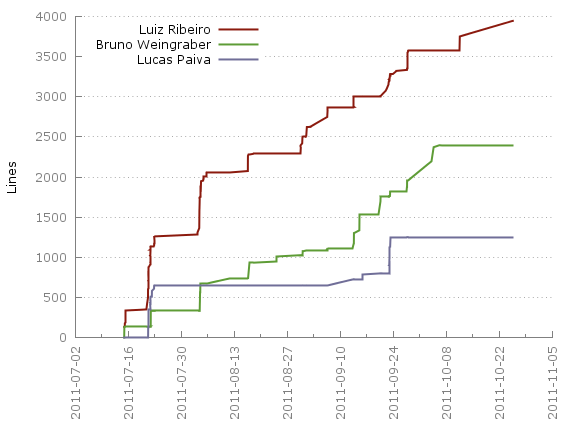
\includegraphics[width=0.7\textwidth]{./plots/lines_of_code_by_author.png}
	\caption[Evolução do número de linhas de código por programador]{Evolução do número de linhas de código do projeto por programador ao longo do processo de desenvolvimento}
	\fonte{Autoria Própria}
	\label{fig:linhascodigoporautor}
\end{figure}

Porém tal metodologia de desenvolvimento distribuído mostrou-se uma excelente opção ao longo do processo, já que frequentemente os horários dos integrantes da equipe se mostraram incompatíveis para reuniões periódicas.

O uso de ferramentas específicas de controle de versão e compartilhamento de código permitiu que fossem utilizada técnicas de revisão de código, as quais permitiram que os integrantes da equipe discutissem detalhes de implementação de código remotamente, sendo tais discussões disponibilizadas para futuros colaboradores. 
Estas revisões de código juntamente com desenvolvimento orientado a testes se mostraram vitais para garantir a qualidade de código, tendo em vista que o desenvolvimento distribuído torna a codificação eficiente porém sujeita a queda neste quesito.
Tais técnicas ajudaram a evitar que fossem introduzidos novos \emph{bugs} ao código já testado e que novos problemas ainda não cobertos pelos testes fosse criados.

A utilização de ferramentas como o Maven permitiu a todos os desenvolvedores utilizarem o editor de sua preferência, já que a codificação tornou-se independente da IDE utilizada.
Esta juntamente com as demais ferramentas utilizadas reforçaram o conceito de \emph{software} livre empregado ao projeto, já que todas elas estão disponíveis sob licenças livres. 

Com base na especificação do \emph{software} e na metodologia discutida, iniciou-se a fase de implementação do projeto (descrita no capítulo \ref{chap:desenv}).
Durante tal fase procurou-se seguir de fielmente a especificação discutida no capítulo \ref{specs}, pois nesta definiu-se grande parte das decisões de arquitetura e técnicas de desenvolvimento, fazendo com que várias dificuldades de implementação fossem previstas e contornadas.
Uma destas foi a interface entre o sistema e o banco de dados, sendo que o modo como esta foi implementada tornou o sistema flexível para futuras modificações quanto ao banco de dados utilizado.

Para quantificar a performance do sistema final, foi realizado testes de \emph{stress}, os quais consistiram em realizar várias requisições paralelas por segundo e observar os tempos de resposta do \emph{software}.
Como mostrado na figura \ref{fig:resposta}, para 20 requisições por segundo o sistema tem um tempo de resposta elevado.
Porém, este teste não caracteriza exatamente um caso real, visto que é improvavel que sejam realizadas 20 requisições por segundo no sistema.
Visando melhorias na performance, foi feita uma proposta futura de projeto na seção \ref{sec:propostas} para tornar o sistema mais eficiente quanto ao tempo de resposta.

\begin{figure}[!htb]
	\centering
	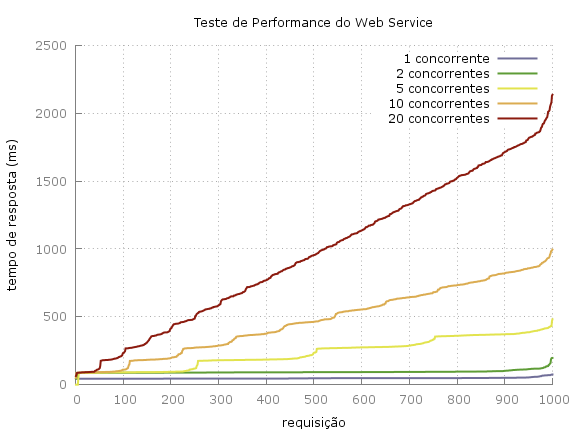
\includegraphics[width=0.7\textwidth]{./plots/stresstests/out.png}
	\caption[Tempo de resposta do \emph{Web Service}]{Tempo de resposta do \emph{Web Service} em função do número de requisições}
	\fonte{Autoria Própria}
	\label{fig:resposta}
\end{figure}

\section{Relação com Engenharia de Computação}
% TODO: Discutir a engenharia, relacionar o trabalho com as disciplinas cursadas, estágios, trabalhos
O desenvolvimento deste projeto agregou muita experiência aos membros da equipe, principalmente pela necessidade de integração de vários conceitos de diversas áreas de conhecimento estudadas ao longo do curso.
Tais conhecimentos englobam as áreas de:
\begin{itemize}
	\item \textbf{Desenvolvimento \emph{web}}: visto que o projeto consiste basicamente em um sistema web.
	\item \textbf{Sistemas distribuídos}: por ser um sistema voltado à \emph{web}, este é um sistema distribuído, sendo aplicáveis os conceitos de arquitetura cliente-servidor e controle de concorrência.
	\item \textbf{Teoria dos Grafos}: a abstração utilizada para abordar o problema envolve a modelagem do mesmo sob a forma de um grafo.
	\item \textbf{Algoritmos}: a implementação do sistema exigiu uma análise dos algoritmos existentes para abordar o problema em questão, assim como a modificação dos mesmos para adaptá-los ao domínio do problema.
	\item \textbf{Estruturas de dados}: para melhorar a performance do sistema, foi de grande importância a escolha cuidadosa das estruturas de dados a serem utilizadas na implementação dos algoritmos.
	\item \textbf{Bancos de dados}: uso de conceitos de transações no banco de dados para grafos empregado ao sistema, bem como a decisão de qual tipo de banco de dados e qual sistema gerenciador de banco de dados deveria ser utilizado no projeto.
	\item \textbf{Engenharia de \emph{software}}: através do uso e adaptação de diversos conceitos, como métodos ágeis, desenvolvimento orientado a testes, revisão de código, uso de sistemas de controle de versão, estabelecimento de metas, entre outros.
\end{itemize}

Esta experiência é fundamental para a carreira profissional de um engenheiro de computação, visto que neste projeto foram bem definidas e realizadas as etapas de um processo de engenharia. 
Tais etapas consistiram em: aquisição de base teórica, estudo do conhecimento estabelecido sobre o assunto, definição dos requisitos, projeto da arquitetura do \emph{software}, definição da metodologia utilizada, implementação efetiva do sistema e por último uma análise dos resultados alcançados. 

\section{Propostas Futuras}
\label{sec:propostas}
Tendo em vista a proporção do presente projeto, ainda há muito o que ser feito para melhorar sua qualidade.
As seguintes propostas foram idealizadas:

\begin{itemize}
	\item Melhorar a performance do sistema quanto ao tempo de resposta para requisições concorrentes, visto que atualmente este tempo pode não ser satisfatório para o uso do mesmo escalas maiores, como mostrado no capítulo \ref{chap:result}.
	\item Desenvolver clientes para plataformas móveis como Android, J2ME ou iOS.
	\item Importar e tratar mais informações originárias dos arquivos GTFS, como tarifas e disponibilidade do serviço de acordo com datas e feriados, sendo que esta última já está sendo importada porém não utilizada pela busca no sistema.
	\item Desenhar a rota resultante utilizando o conceito de \emph{shapes} do GTFS, com o intuito de desenhá-la coincidindo com as ruas presentes no mapa.
Esta proposta já está em andamento, sendo que as \emph{shapes} já são importadas para o banco de dados porém não são utilizadas para desenho da rota resultante.
	\item Melhorar o \emph{layout} da interface \emph{web}.
	\item Adicionar novas funcionalidades ao sistema, como suporte a consultas que tem como entrada um horário de chegada ao destino, permitindo que o usuário saiba que horas deve sair da origem para alcançar o destino em um determinado horário, por exemplo.
	\item Implementação de busca multi-objetivo, ou seja, considerar diferentes fatores para minimizar o custo de viagem, como valor da tarifa total e a minimização 		do número de trocas de veículos, desta forma obtendo-se um conjunto de soluções ótimas para sugerir diferentes rotas ao usuário.
	\item Adquirir os dados de Curitiba, ou de outras cidades brasileiras, para transporte público no formato GTFS, para então implantar o sistema na cidade em questão.
\end{itemize}
